\documentclass[11pt, a4paper, twoside]{article}   	% use "amsart" instead of "article" for AMSLaTeX format

\usepackage{geometry}                		% See geometry.pdf to learn the layout options. There are lots.
\usepackage{pdfpages}
\usepackage{caption}
\usepackage{minted}
\usepackage[german]{babel}			% this end the next are needed for german umlaute
\usepackage[utf8]{inputenc}
\usepackage{color}
\usepackage{graphicx}
\usepackage{titlesec}
\usepackage{fancyhdr}
\usepackage{lastpage}
\usepackage{hyperref}
% http://www.artofproblemsolving.com/wiki/index.php/LaTeX:Symbols#Operators
% =============================================
% Layout & Colors
% =============================================
\geometry{
   a4paper,
   total={210mm,297mm},
   left=20mm,
   right=20mm,
   top=20mm,
   bottom=30mm
 }	

\definecolor{myred}{rgb}{0.8,0,0}
\definecolor{mygreen}{rgb}{0,0.6,0}
\definecolor{mygray}{rgb}{0.5,0.5,0.5}
\definecolor{mymauve}{rgb}{0.58,0,0.82}

\setcounter{secnumdepth}{4}


% the default java directory structure and the main packages
\newcommand{\srcDir}{../src/main/java}
\newcommand{\srcTestDir}{../src/test/java}
\newcommand{\resourcesTestDir}{../src/test/resources}
\newcommand{\mainPackageDir}{\srcDir/at/fh/ooe/swe4/collections}
\newcommand{\mainTestPackageDir}{\srcTestDir/at/fh/ooe/swe4/test/collections}
\newcommand{\binTreeTests}{\mainTestPackageDir/binarySearchTreeSet}
\newcommand{\commonTreeTests}{\mainTestPackageDir/common/parametrized}
\newcommand{\nmkTreeTests}{\mainTestPackageDir/twoThreeFourTreeSet}
\newcommand{\imagesDir}{images}
% the default subsection headers
\newcommand{\ideaSection}{Lösungsidee}
\newcommand{\sourceSection}{Source-Code}
\newcommand{\testSection}{Tests}

% =============================================
% Code Settings
% =============================================
\newenvironment{code}{\captionsetup{type=listing}}{}
\newmintedfile[javaSourceFile]{java}{
	linenos=true, 
	frame=single, 
	breaklines=true, 
	tabsize=2,
	numbersep=5pt,
	xleftmargin=10pt,
	baselinestretch=1,
	fontsize=\footnotesize
}
\newmintinline[inlineJava]{java}{}
\newminted[javaSource]{java}{
	breaklines=true, 
	tabsize=2,
	autogobble=true,
	breakautoindent=false
}
\newmintedfile[xmlSourceFile]{xml}{
	linenos=true, 
	frame=single, 
	breaklines=true, 
	tabsize=2,
	numbersep=5pt,
	xleftmargin=10pt,
	baselinestretch=1,
	fontsize=\footnotesize
}
\newmintedfile[propertiesFile]{properties}{
	linenos=true, 
	frame=single, 
	breaklines=true, 
	tabsize=2,
	numbersep=5pt,
	xleftmargin=10pt,
	baselinestretch=1,
	fontsize=\footnotesize
}
% =============================================
% Page Style, Footers & Headers, Title
% =============================================
\title{Übung 3}
\author{Thomas Herzog}

\lhead{Übung 3}
\chead{}
\rhead{
\includegraphics[scale=0.10]{FHO_Logo_Students.jpg}}

\lfoot{S1310307011}
\cfoot{}
\rfoot{ \thepage / \pageref{LastPage} }
\renewcommand{\footrulewidth}{0.4pt}
% =============================================
% D O C U M E N T     C O N T E N T
% =============================================
\pagestyle{fancy}
\begin{document}
\setlength{\headheight}{15mm}
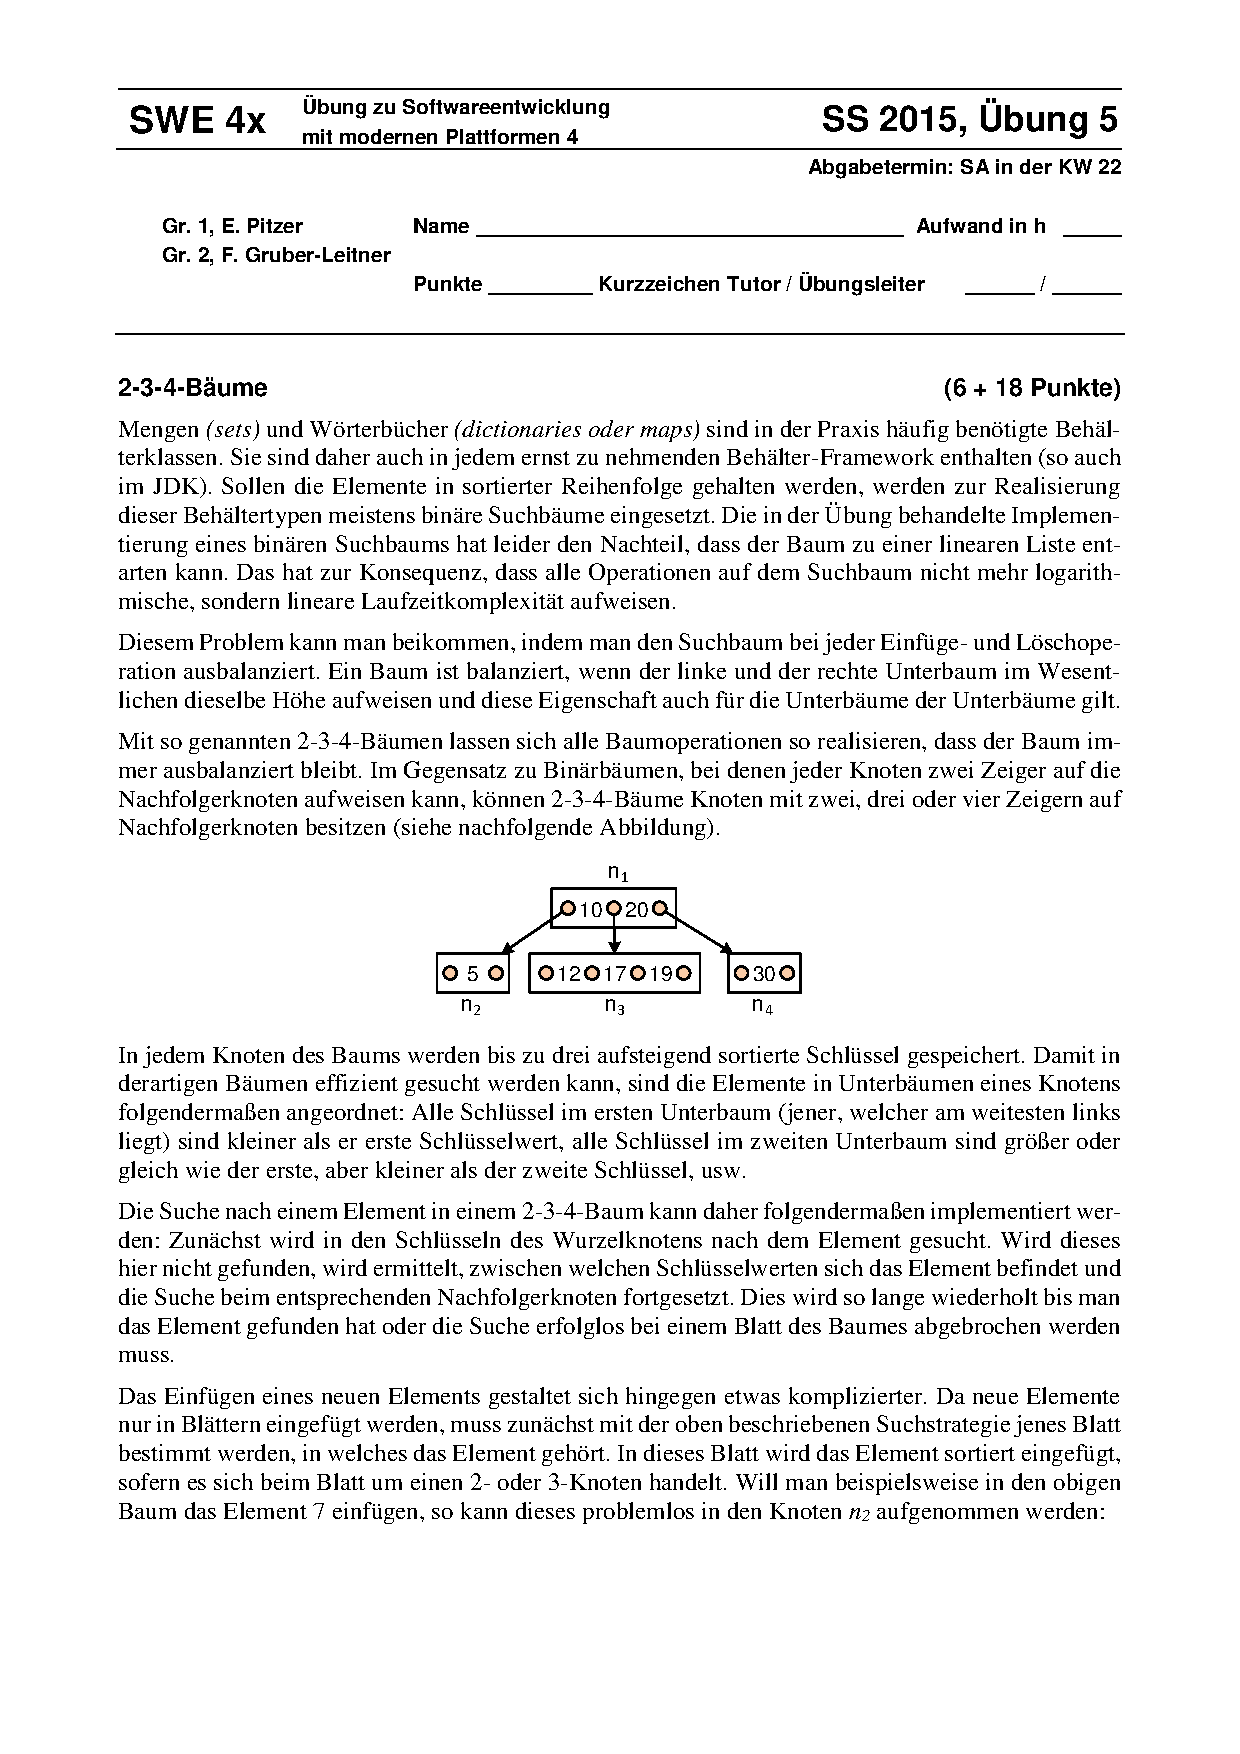
\includepdf[pages={1-3}]{Swe4xA05-BB.pdf}
{\color{myred}
	\section
		{Binäre Suchbäume}
}

\subsection{\ideaSection}
Folgend ist die Dokumentation für die Aufgabenstellung binäre Suchbäume angeführt. \\
Wie verlangt soll der binäre Suchbaum aus der Übung erweitert werden, wobei jedoch die bestehende Implementierung verbessert werden soll, z.B.: über eine abstrakte Superklasse, die Methoden wie \inlineJava{boolean contains(Object); Comparator<T> comparator();} implementiert.\\
Des Weiteren soll eine Methode \inlineJava{compareElemets(T o1, T o2);} implementiert werden, die entweder, bei zu Verfügung stehender \inlineJava{Comparator<T>} Implementierung, an diesen delegiert oder die Elemente auf \inlineJava{Comparable<T>} casted und so den Vergleich durchführt.
Ansonsten ist die bestehende Implementierung wie verlangt zu erweitern.\\

Bezüglich des 2-3-4 Baums sei angemerkt, dass sich hier das Iterieren über den Baum als Herausforderung herausstellen könnte, da der gewöhnliche Ansatz (left, right) nicht anwendbar ist.\\
Hier ist es erforderlich das man immer zum Parent zurückkehrt und seine nächste Child Node besucht und hier wieder solange nach links geht bis man zur letzten Node kommt.\\
Diese kann man wieder ausgeben und man muss denselben Ansatz bei dessen Parent anwenden, solange bis man alle Nodes des Baums besucht hat.\\
Daher scheint es mir sinnvoll hier über ein Model zu arbeiten, und eine doppelte Verkettung der Nodes (\inlineJava{parent < - > child}) anzuwenden. Die tatsächlichen Nodes dürfen nicht geändert werden, daher muss hier über die Iteratoren deren Children und Keys zu arbeiten, die vom Model verwaltet werden sollen.\\\\
Beim Durchwandern des Baums sollten folgende Zustände auftreten:\\
\begin{enumerate}
	\item Node hat keine Kinder, daher können alle seine Keys ausgegeben werden
	\item Node hat Children daher soll der nächste Key ausgegeben werden und zur nächsten Child Node gewechselt werden, sofern die Node (Parent) aus dem Stack kommt. (Achtung: Parent gehört wieder am Stack)
	\item Hat diese Node wieder Kinder, so muss wieder zu seiner kleinsten Node gewandert werden.
	\item Die Parents müssen beim Besuch des Child darüber Informiert werden, das dieser vollständig besucht wurde. (Über Model und doppelte Verkettung)
\end{enumerate}
Für Implementierungsdetails sei auf den Source verwiesen.\\\\
Für die Tests soll wieder die Testsuite aus der letzten Übung verwendet werden, wobei in dieser Dokumentation auf dessen Source und Implementierung nicht mehr genauer eingegangen werden soll. Sie soll als Third-Party-Library angesehen werden.\\\\
Da sehr viel Dokumentation in Form von Java-Doc vorhanden ist, sei generell auf diese Dokumentation verwiesen.

\newpage
\subsection{\sourceSection (Implementation)}
Folgend ist der Source der Implementierungen der Übung angeführt.\\

\subsubsection{SortedSet.java}
Folgend ist das Interfaces \inlineJava{SortedSet<T>} angeführt, welches aus der Aufgabenstellung hervorging.
\begin{code}
	\caption{SortedSet.java}
	\javaSourceFile{\mainPackageDir/api/SortedSet.java}
\end{code}
\newpage

\subsubsection{SortedTreeSet.java}
Folgend ist das Interfaces \inlineJava{SortedTreeSet<T>} angeführt, welches aus der Aufgabenstellung hervorging und eine Erweiterung des Interfaces \inlineJava{SortedSet<T>} darstellt.
\begin{code}
	\caption{SortedTreeSet.java}
	\javaSourceFile{\mainPackageDir/api/SortedTreeSet.java}
\end{code}

\subsubsection{Node.java}
Folgend ist das Interfaces \inlineJava{Node<T>} angeführt, welches als Marker Interface für die Tree Nodes fungiert, damit die abstrakte Klasse \inlineJava{AbstractSortedSet<T, M extends Model<T> alle Node Typen aufnehmen kann. Dies ist möglich, da es keine Methoden der Nodes benötigt.}
\begin{code}
	\caption{Node.java}
	\javaSourceFile{\mainPackageDir/api/Node.java}
\end{code}
\newpage

\subsubsection{AbstractSortedSet.java}
Folgend ist das Interfaces \inlineJava{AbstractSortedSet<T>} angeführt, welches als abstrakte Klasse implementiert wurde. Sie implementiert ebenfalls eine \inlineJava{compareElements(T o1, T o2)} Methode, die Elemente entweder mit einem zur Verfügung gestellten \inlineJava{Comparator<T>} oder mittels natürlicher Ordnung ordnet.
\begin{code}
	\caption{AbstractSortedSet.java}
	\javaSourceFile{\mainPackageDir/api/AbstractSortedSet.java}
\end{code}
\newpage

\subsubsection{NullSafeComparableComparator.java}
Folgend ist Implementierung eines Null-Safe \inlineJava{COmparator<T>} angeführt, welcher als Default für die \inlineJava{compareElements{T o1, T o2}} verwendet wird. 
\begin{code}
	\caption{NullSafeComparableComparator.java}
	\javaSourceFile{\mainPackageDir/comparator/NullSafeComparableComparator.java}
\end{code}
\newpage

\subsubsection{EnumerationConstants.java}
Folgend ist Implementierung einer Konstanten Klasse angeführt, welche die Enumeration Klassen Spezifikationen enthält. Es sollten für diese einfachen Enumerationen keine eigenen Klassendateien erstellt werden.
\begin{code}
	\caption{EnumerationConstants.java}
	\javaSourceFile{\mainPackageDir/constants/EnumerationConstants.java}
\end{code}
\newpage

\subsubsection{BinaryTreeNode.java}
Folgend ist Implementierung des Tree Node Models angeführt, welches als Wrapper für die verwalteten Keys fungiert. Dieses Model ist für einen binären Suchbaum (2 Nachfolgeknoten) implementiert worden.
\begin{code}
	\caption{BinaryTreeNode.java}
	\javaSourceFile{\mainPackageDir/model/BinaryTreeNode.java}
\end{code}
\newpage

\subsubsection{NMKTreeNode.java}
Folgend ist Implementierung des Tree Node Models angeführt, welches als Wrapper für die verwalteten Keys fungiert. Dieses Model ist für einen n-m-k Suchbaum, in unserem Fall einen 2-3-4 Baum, implementiert worden.
\begin{code}
	\caption{NMKTreeNode.java}
	\javaSourceFile{\mainPackageDir/model/NMKTreeNode.java}
\end{code}
\newpage

\subsubsection{BinarySearchTreeSet.java}
Folgend ist Implementierung des binären Suchbaums angeführt. Der \inlineJava{Iterator<T>} wurde als innere Klasse implementiert.
\begin{code}
	\caption{BinarySearchTreeSet.java}
	\javaSourceFile{\mainPackageDir/impl/BinarySearchTreeSet.java}
\end{code}
\newpage

\subsubsection{TwoThreeFourTreeSet.java}
Folgend ist Implementierung des 2-3-4 Baums angeführt. Der \inlineJava{Iterator<T>} wurde als externe Klasse implementiert.
\begin{code}
	\caption{TwoThreeFourTreeSet.java}
	\javaSourceFile{\mainPackageDir/impl/TwoThreeFourTreeSet.java}
\end{code}
\newpage

\subsubsection{NMKTreeIterator.java}
Folgend ist Implementierung des n-m-k \inlineJava{Iterator<T>} angeführt. Dieser Iterator sollte mit 1-2-3 genauso wie mit 2-3-4 oder irgendeiner anderen Art funktionieren, solange sich die Baumvariationen wie ein 2-3-4 Baum verhalten nur mit andere Node/Key Anzahl.
\begin{code}
	\caption{NMKTreeIterator.java}
	\javaSourceFile{\mainPackageDir/iterator/NMKTreeIterator.java}
\end{code}
\newpage

\newpage
\subsection{\sourceSection (Tests)}
Folgend ist der Source der Tests der Übung angeführt.\\

\subsubsection{BinarySearchTreeTestDataProducer.java}
Folgend ist die Implementierung eines Tests Data Producers angeführt, welche die Testdaten für binäre Test Klassen zur Verfügung stellt, wobei es sich hierbei um 2 selbst aufgebaute Bäume handelt.
\begin{code}
	\caption{BinarySearchTreeTestDataProducer.java}
	\javaSourceFile{\binTreeTests/api/BinarySearchTreeTestDataProducer.java}
\end{code}
\newpage

\subsubsection{IteratorValidTest.java}
Folgende Testklasse testet den Iterator des binären Suchbaums und wendet dazu parametrisierte Tests an, die mit den produzierten Testdaten das iterieren testen.
\begin{code}
	\caption{IteratorValidTest.java}
	\javaSourceFile{\binTreeTests/impl/parametrized/IteratorValidTest.java}
\end{code}
\newpage

\subsubsection{AddTest.java}
Folgende Testklasse testet das hinzufügen von Elementen in den Baum.
\begin{code}
	\caption{AddTest.java}
	\javaSourceFile{\binTreeTests/impl/AddTest.java}
\end{code}
\newpage

\subsubsection{IteratorTest.java}
Folgende Testklasse testet den Iterator auf Fehlerverhalten.
\begin{code}
	\caption{IteratorTest.java}
	\javaSourceFile{\binTreeTests/impl/IteratorTest.java}
\end{code}
\newpage

\subsubsection{SortedTreeSetTest.java}
Folgende Testklasse testet das Interface \inlineJava{SortedTreeSet<T>} über einen parametrisierten Test, der beide Implementierungen mit und ohne \inlineJava{Comparator<T>} testet.
\begin{code}
	\caption{SortedTreeSetTest.java}
	\javaSourceFile{\commonTreeTests/SortedTreeSetTest.java}
\end{code}
\newpage

\subsubsection{TwoThreeFourTreeSetDataProducer.java}
Folgend ist die Implementierung eines Testdaten Producers angeführt, welcher Testdaten produziert, also fertig und manuell aufgebaute Bäume.
\begin{code}
	\caption{TwoThreeFourTreeSetDataProducer.java}
	\javaSourceFile{\nmkTreeTests/api/TwoThreeFourTreeSetDataProducer.java}
\end{code}
\newpage

\subsubsection{IteratorValidTest.java}
Folgende Testklasse testen den Iterator über einen parametrisierten Test, der die Tesdaten zur Verfügung stellt.
\begin{code}
	\caption{IteratorValidTest.java}
	\javaSourceFile{\nmkTreeTests/impl/parametrized/IteratorValidTest.java}
\end{code}
\newpage

\subsubsection{AddTest.java}
Folgende Testklasse testen die Methode \inlineJava{boolean add(T el);}der 2-3-4 Baum Implementierung.
\begin{code}
	\caption{AddTest.java}
	\javaSourceFile{\nmkTreeTests/impl/AddTest.java}
\end{code}
\newpage

\subsubsection{IteratorTest.java}
Folgende Testklasse testet das Fehlerverhalten der Iterator Implementierung.
\begin{code}
	\caption{IteratorTest.java}
	\javaSourceFile{\nmkTreeTests/impl/IteratorTest.java}
\end{code}
\newpage

\subsection{\testSection}
Folgend sind die Testergebnisse angeführt.\\
Da es wenig sinnvolle Information zu loggen gab, sei hier nur ein Screenshot der JUnit Tests angeführt. Für Informationen bezüglich der Tests sei auf den Test Source verwiesen.\\

\begin{figure}[h]
	\centering
	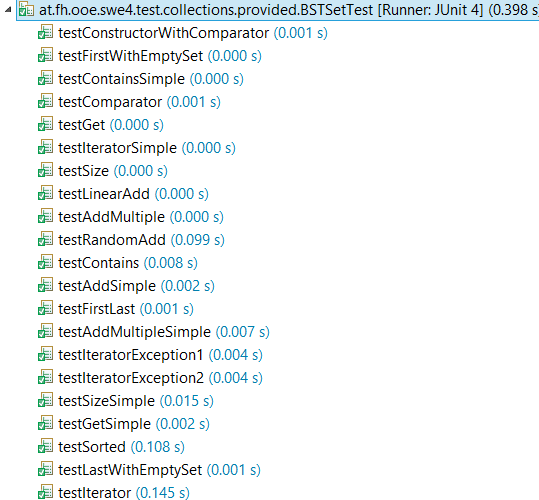
\includegraphics[scale=1]{\imagesDir/provided_1.PNG}
	\caption
	{Diese Abbildung zeigt die Testergebnisse des \inlineJava{BinarySearchTreeSet<T>} der zur Verfügung gestellten Tests}
\end{figure}
\newpage

\begin{figure}[h]
	\centering
	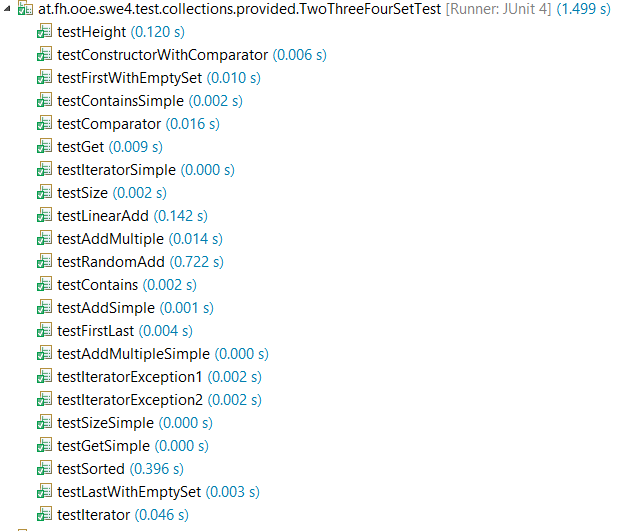
\includegraphics[scale=1]{\imagesDir/provided_2.PNG}
	\caption
	{Diese Abbildung zeigt die Testergebnisse des \inlineJava{TwoThreeFourSortedTreeSet<T>} der zur Verfügung gestellten Tests}
\end{figure}
\newpage 

\begin{figure}[h]
	\centering
	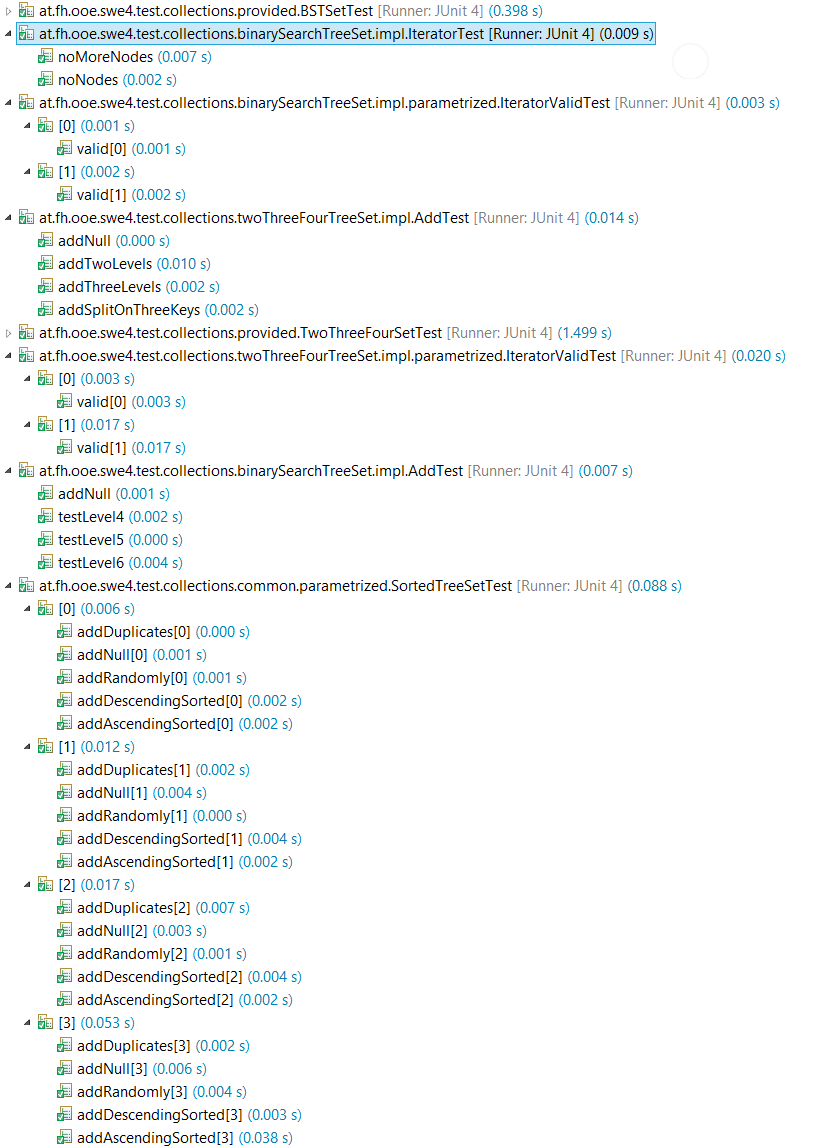
\includegraphics[scale=1]{\imagesDir/mine_1.PNG}
	\caption
	{Diese Abbildung zeigt die Testergebnisse der eigenen Tests}
\end{figure}
\newpage

\begin{figure}[h]
	\centering
	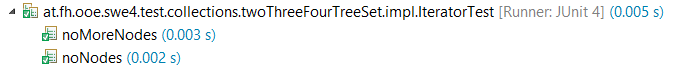
\includegraphics[scale=1]{\imagesDir/mine_2.PNG}
	\caption
	{Der zweite Teil der eigenen Tests}
\end{figure}
\newpage 
\end{document}  